% 2009 年江西卷文科第 9 题：四面体 ABCD 与正方形截面 PQMN。
% 来源 PDF：普通高考/2009/2009江西文.pdf，SHA-256 468ed0d312446a29e8cdaebe70fab4f803741b0b542cd991781b2f13fed5168f。
% 原页：第 1 页（A3 三栏）第 1 栏，书页码 535。
% 重绘依据：原图 A 在顶点，B 在左下、C 在右下，D 在四边形内部（被遮挡，连 AD、BD、CD 为虚线）；
%   截面四顶点 P∈AB、N∈AD、M∈DC、Q∈BC，PQ∥AC、PN∥BD，取 AP/AB=0.59、BQ/BC=0.41 使投影两侧近似等长。
%   原图 P-N、P-Q 为实线，N-M、M-Q 为虚线。
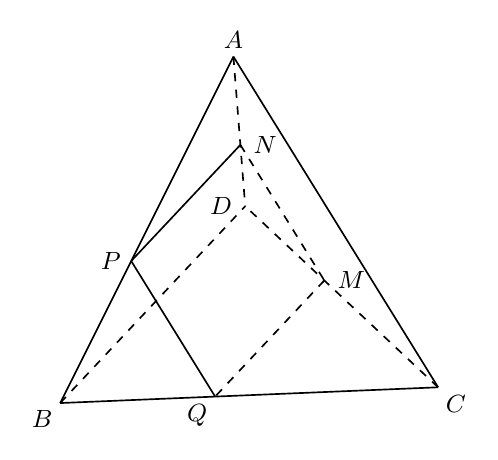
\begin{tikzpicture}[scale=1.0, semithick, every node/.style={inner sep=1.5pt, font=\small}]
  \coordinate (A) at (0,4.40);
  \coordinate (B) at (-2.20,0);
  \coordinate (C) at (2.60,0.20);
  \coordinate (D) at (0.15,2.50);
  \coordinate (P) at (-1.298,1.804);
  \coordinate (Q) at (-0.232,0.082);
  \coordinate (N) at (0.0885,3.279);
  \coordinate (M) at (1.1545,1.557);

  % 四面体的棱：实线为可见棱，虚线为被遮挡棱
  \draw (A) -- (B);
  \draw (A) -- (C);
  \draw (B) -- (C);
  \draw[dashed] (A) -- (D);
  \draw[dashed] (B) -- (D);
  \draw[dashed] (C) -- (D);

  % 正方形截面 PQMN：靠前的两条边实线，靠后的两条边虚线
  \draw (P) -- (N);
  \draw (P) -- (Q);
  \draw[dashed] (N) -- (M);
  \draw[dashed] (M) -- (Q);

  \node[above=1pt] at (A) {$A$};
  \node[below left=1pt] at (B) {$B$};
  \node[below right=1pt] at (C) {$C$};
  \node[left=2pt] at (P) {$P$};
  \node[below left=1pt] at (Q) {$Q$};
  \node[right=3pt] at (N) {$N$};
  \node[right=3pt] at (M) {$M$};
  \node[left=3pt] at (D) {$D$};
\end{tikzpicture}
